% Section 4: Experiment 1 — Small Library (v2) (~1.5 pages)

\subsection{Setup}

We run 250 tasks across 5 themes (ML Fundamentals, Agent Architectures, Multi-Agent Systems, Evaluation Methods, Retrieval Systems) with 100 easy, 100 medium, and 50 hard tasks.
The skill library contains 50 meta-skills across 5 domains (research, creative, synthesis, evaluation, operational).
All four conditions execute the same tasks in the same order, yielding 1,000 total episodes.

The LLM is MiniMax M2.5 (temperature${=}$0.7), chosen for cost efficiency under budget constraints.
Embeddings use Qwen3-Embedding-0.6B (1,024 dimensions, 70.7 MTEB) running locally.
Each task allows up to 35 LLM turns (steps), with a metacognitive synthesis nudge injected at 60\% budget consumption.

\subsection{Results: Token Efficiency}

Table~\ref{tab:v2_results} presents the main results.
All three feedback conditions achieve statistically significant token reductions compared to the control.

\begin{table}[t]
\centering
\small
\begin{tabular}{lrrrr}
\toprule
\textbf{Cond.} & \textbf{Mean Tok.} & \textbf{Med.} & \textbf{Multi\%} & \textbf{$\Delta$ vs C1} \\
\midrule
C1 & 6,481 & 3,116 & 11.6\% & --- \\
C2 & 3,906 & 2,977 & 5.6\% & $-$39.7\% \\
C3 & 3,526 & 2,930 & 4.0\% & $-$45.6\% \\
C4 & 3,256 & 2,845 & 3.2\% & $-$49.8\% \\
\bottomrule
\end{tabular}
\caption{Experiment~1 (v2) main results. Token reduction is relative to C1 mean. Bootstrap 95\% CIs (10,000 resamples): C1 vs.\ C2 $p=0.012$, C1 vs.\ C3 $p<0.001$, C1 vs.\ C4 $p<0.001$; all survive Holm--Bonferroni correction for 3 C1-vs-treatment comparisons. Parametric tests are inappropriate given C1 SD$=$24{,}746 vs.\ C4 SD$=$2{,}037.}
\label{tab:v2_results}
\end{table}

A notable divergence exists between mean and median reductions.
The median gap is only 8.7\% (C1$=$3{,}116 vs.\ C4$=$2{,}845), while the mean gap is 49.8\%.
This indicates that the treatment effect is concentrated in the upper tail of the token distribution, specifically in multi-step episodes (Figure~\ref{fig:v2_token_boxplot}).

\subsection{Mechanism: Multi-Step Prevention}
\label{sec:multistep}

The primary observation from Experiment~1 is that all efficiency gains come from reducing multi-step episodes, not from improving single-step performance.

Single-step episodes consume ${\sim}$2,950 tokens across all four conditions ($<$1\% spread).
The LLM produces nearly identical responses when it does not enter an iterative reasoning loop, regardless of which skills were retrieved or whether a feedback rubric was present.

Multi-step episodes tell a different story.
C1 triggers multi-step reasoning in 11.6\% of tasks, with each multi-step episode consuming an average of 33,256 tokens.
C4 triggers multi-step reasoning in only 3.2\% of tasks (12,784 tokens each when triggered).
The feedback rubric acts as a metacognitive anchor: by requiring the LLM to evaluate retrieval quality, it structures the response in a way that prevents exploration spirals.

Put differently, even without adaptive retrieval, simply appending a feedback rubric to an LLM system may reduce multi-step failures and token consumption.

\begin{figure}[t]
\centering
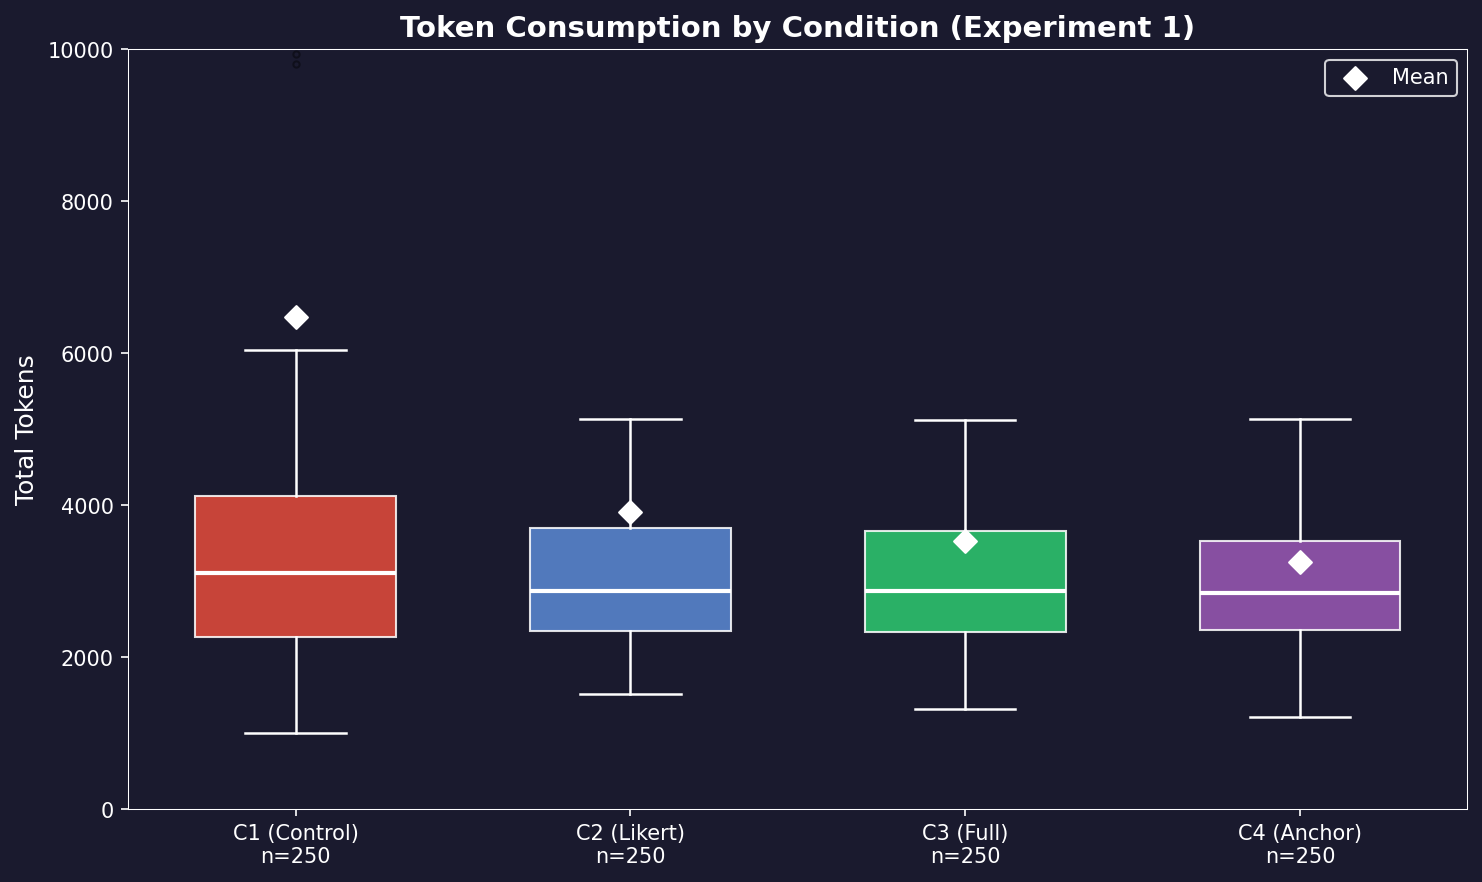
\includegraphics[width=\columnwidth]{../results/figures/fig1_v2_token_boxplot.png}
\caption{Token consumption distributions by condition (v2). The heavy right tail of C1 reflects multi-step episodes (11.6\% of tasks), which are progressively eliminated in treatment conditions. The treatment effect operates primarily through tail compression rather than location shift.}
\label{fig:v2_token_boxplot}
\end{figure}

\subsection{Bandit Convergence}
\label{sec:convergence}

Thompson Sampling produces distinct convergence patterns across conditions.

\textbf{C2 (Likert feedback)} converges to the importance-heavy preset (posterior mean 0.633 by the final quartile), with the balanced preset (Park et al.\ default) ranking near the bottom.
\textbf{C3 (Likert + explanation embeddings)} converges to the relevance-importance preset (0.616) and converges faster than C2 (by Q2 vs.\ Q3), with wider posterior spread (0.151 vs.\ 0.106).
The explanation embeddings stored in C3 appear to strengthen the reward signal.
\textbf{C4 (qualitative anchors)} shows no convergence: all arms hover near 0.42 (spread $=$0.014).
Despite achieving the best token efficiency, C4's anchor embedding parser compresses reward variance 3.6$\times$ relative to Likert parsing, leaving insufficient signal for the bandit to differentiate arms.

The C4 paradox, best efficiency with no weight learning, is the key diagnostic finding.
It demonstrates that the token efficiency gains in Experiment~1 are driven by the \emph{rubric prompt effect} (present in all treatment conditions), not by the \emph{adaptive retrieval effect} (present only when the bandit converges).
This has three implications: (1)~the rubric prompt effect is \emph{largely independent of} retrieval weight adaptation, providing its benefit independently of whether the bandit converges; (2)~embedding-based reward inference (C4's anchor parser) trades off signal fidelity for ecological validity: the 3.6$\times$ variance compression produces smoother but less informative rewards; (3)~future work on adaptive retrieval must control for the rubric prompt confound, isolating weight learning effects from metacognitive anchoring effects.

\subsection{Diagnosis: Why Weight Learning Didn't Improve Retrieval}

\paragraph{Skill overlap.}
Pairwise Jaccard similarity of the top-5 retrieved skills between conditions: C1 vs.\ C2 $= 0.904$, C1 vs.\ C3 $= 0.909$, C1 vs.\ C4 $= 0.848$.
Different weight presets change the \emph{scores} of skills but not the \emph{rankings}: the same ${\sim}$6 meta-skills dominate 86\% of all retrievals regardless of weights (Appendix Figure~\ref{fig:skill_heatmap}).

\paragraph{Root cause: dimension saturation.}
The recency dimension is near-saturated at ${\sim}$0.95 (most skills were used recently in a sequential experiment) and importance at ${\sim}$0.96 (Laplace smoothing with high success rate).
Only relevance (${\sim}$0.43) has meaningful variance (see Figure~\ref{fig:v3_jaccard_trajectory} for the trajectory across both experiments).
With two of three dimensions effectively constant, weight changes cannot produce different skill orderings.

\paragraph{Two independent effects.}
We identify two separable mechanisms:
\begin{enumerate}
\item \textbf{Rubric prompt effect} (all treatment conditions): The feedback rubric structures the LLM's response, preventing multi-step spirals. This is a prompt engineering effect, not a retrieval effect.
\item \textbf{Adaptive retrieval effect} (C2/C3 only): Thompson Sampling converges, but convergence does not change retrieved skills due to dimension saturation.
\end{enumerate}
C4 achieves effect~1 without effect~2's overhead, explaining its paradoxical advantage.

\paragraph{Per-difficulty breakdown.}
The rubric prompt effect scales with task difficulty: easy tasks show 6--15\% token reduction, medium tasks 30--45\%, and hard tasks 60--70\%.
This is consistent with the multi-step prevention mechanism: harder tasks are more likely to trigger reasoning spirals, so preventing those spirals yields larger savings.
